\documentclass{article}
\usepackage[francais]{babel}
\usepackage[utf8]{inputenc}
\usepackage{xcolor}
\usepackage[pdftex]{graphicx}
\usepackage{listings}
\usepackage{amsmath}
\usepackage[a4paper,includeheadfoot,margin=2.54cm]{geometry}
\usepackage{amsfonts}
\usepackage{fancyhdr}
\usepackage{titling}
\usepackage{algorithm}
\usepackage{algpseudocode}
\usepackage{hyperref}

\pagestyle{fancy}
\fancyhf{}
\fancyhead[LE,RO]{\theauthor}
\fancyhead[RE,LO]{\thetitle}
\fancyfoot[CE,CO]{\leftmark}
\fancyfoot[LE,RO]{\thepage}

\usepackage[thinlines]{easytable}

\title{Rapport de projet: Gomoku}
\author{Quentin Garrido, Antoine Gélin, Kévin Lor}
\date{22 février 2019}

\begin{document}

\maketitle
\tableofcontents
\pagebreak

\section{Introduction}

Le but de ce projet est de réaliser une "intelligence artificielle" pouvant jouer contre un humain au gomoku.\\
Nous avons choisi d'utiliser un plateau de 8$	imes$8 et une victoire avec l'alignement de 5 pions de même couleur.\\
Nous avons programmé en C++ afin d'avoir un langage familier à tout le groupe et qui nous permet d'utiliser
certaines représentations pour nos structures de données que nous verrons par la suite.\\
L'un des membres du groupe s'intéressant au moteurs d'échecs et ayant une connaissance des algorithmes utilisés
nous avons transposé ces méthodes vers le gomoku, qui possède les même caractéristique en étant plus simple.\\

Le projet à été réalisé à travail égal par tous les membres du groupe en suivant la répartition suivante:
\begin{itemize}
	\item Quentin Garrido: Structures de données et parcours des coups
	\item Antoine Gélin: Évaluation des coups et réalisation des tests
	\item Kévin Lor: Évaluation des coups et gestion de la mémoire
\end{itemize}

\section{Utilisation}

Tout le code source est disponible à l'adresse suivante : \textit{https://github.com/garridoq/gomoku}.\\

Tout les éxécutables devraient vous être fournis dans le mail et devraient fonctionner sans devoir
les recompiler. Dans le cas contraire voici la démarche à suivre:\\

Afin de pouvoir compiler les exécutables il faut être sous Linux et avoir g++ d'installé sur la machine.\\
La norme utilisée est le C++14 pour tout le programme.\\

Une fois le code source obtenu il faudra exécuter la commande suivante pour compiler les exécutables:
\begin{lstlisting}[language=bash]
	> make
\end{lstlisting}

Tout en étant dans le dossier du code source.\\

Vous obtiendrez plusieurs exécutables de test, ayant un nom comme \textit{test\_*}.\\
Vous aurez aussi un fichier principal \textit{main} qui vous permettra de jouer contre l'IA.

\pagebreak
%==============================================================================
\section{Structures de données}
\subsection{Représentation du plateau}

Pour représenter le plateau nous n'avons pas utilisé de tableau mais des \textit{bitboards} qui
sont la représentation d'un plateau avec chaque case repréenté par un bit, ainsi si elle est
occupée le bit vaudra 1 et 0 sinon.\\
Le bit de poids fort sera le coin en haut à gauche de notre plateau et celui de poids faible le coin 
en bas à droite. Nous avons alors la représentation suivante pour un plateau de 8$\times$8:

\begin{figure}[!hbt]
	\centering
	\begin{TAB}(e, 0.5cm, 0.5cm){|c|c|c|c|c|c|c|c|}{|c|c|c|c|c|c|c|c|}
		 &  &  &  &  &  &  &  \\
		 &  &  &  &  & X &  &  \\
		 &  & X & X &  &  &  &  \\
		 &  &  &  & X &  &  &  \\
		 &  &  &  &  & X &  &  \\
		 &  &  &  &  &  &  &  \\
		 &  &  &  &  &  &  &  \\
		 &  &  &  &  &  &  &  
	\end{TAB}\hspace{0.5cm}
	\begin{TAB}(e, 0.5cm, 0.5cm){|c|c|c|c|c|c|c|c|}{|c|c|c|c|c|c|c|c|}
		0 &0  &0  &0  &0  &0  &0  &0  \\
		0 &0  &0  &0  &0  & 1 &0  &0  \\
		0 &0  & 1 & 1 &0  &0  &0  &0  \\
		0 &0  &0  &0  & 1 &0  &0  &0  \\
		0 &0  &0  &0  &0  &1  &0  &0  \\
		0 &0  &0  &0  &0  &0  &0  &0 \\ 
		0 &0  &0  &0  &0  &0  &0  &0 \\
		0 &0  &0  &0  &0  &0  &0  &0 \\ 
	\end{TAB}
	
	\begin{TAB}(e, 0.5cm, 0.5cm){|c|c|c|c|c|c|c|c|}{|c|c|c|c|c|c|c|c|}
		 &  &  &  &  &  &  &  \\
		 &  &  &  &  &  &  &  \\
		 &  &  &  &O  &  &  &  \\
		 & O &  &  &  &O  &  &  \\
		 &  & O & O &  &  &  &  \\
		 &  &  &  &  &  &  &  \\
		 &  &  &  &  &  &  &  \\
		 &  &  &  &  &  &  &  
	\end{TAB}\hspace{0.5cm}
	\begin{TAB}(e, 0.5cm, 0.5cm){|c|c|c|c|c|c|c|c|}{|c|c|c|c|c|c|c|c|}
		0 &0  &0  &0  &0  &0  &0  &0  \\
		0 &0  &0  &0  &0  &0  &0  &0  \\
		0 &0  &0  &0  &1  &0  &0  &0  \\
		0 & 1 &0  &0  &0  &1  &0  &0  \\
		0 &0  &1  &1  &0  &0  &0  &0  \\
		0 &0  &0  &0  &0  &0  &0  &0  \\
		0 &0  &0  &0  &0  &0  &0  &0  \\
		0 &0  &0  &0  &0  &0  &0  &0  
	\end{TAB}
	\caption{Représentation d'un plateau avec les bitboards associés}
\end{figure}

Ainsi nous gagnons en mémoire, une position ne nécessite plus que 128bits pour être stockée
et nous béneficions de l'implémentation en hardware du décalage des nombres, ce qui nous fera
gagner de la rapidité à l'évaluation des coups.\\

C'est ce choix de représentation qui a motivé notre choix d'utiliser le C++ pour le projet.
En effet il est un des rares langages qui nous permet d'accéder à chaque bits individuellement
d'un nombre et de réaliser des opérations logiques bit par bit. \\
Pour représenter un plateau de $n$x$n$ il nous faut $n^2$ bits d'où le choix du plateau 8$\times$8
car un entier au delà de 64bits est plus dur à représenter en C++.\\

Cette réprésentation va aussi simplifier l'évaluation des coups en elle même car il sera
plus simple de réaliser un parcours de motif (pattern) en décalant les bits de ce dernier.

\pagebreak
\subsection{Pattern}

Les patterns seront un élément clef de notre programme car nous permettrons d'évaluer une position.\\
Ils seront eux aussi représentés par des \textit{bitboards} et nous aurons aussi l'information sur leur
\textit{hauteur} et \textit{largeur}.Afin de faciliter le parcours du motif sur le plateau de jeu, nous
ferons commencer les motifs le plus en haut à gauche possible du plateau.

\begin{figure}[!hbt]
	\centering
	\begin{TAB}(e, 0.5cm, 0.5cm){|c|c|c|c|c|c|c|c|}{|c|c|c|c|c|c|c|c|}
		 &  &  &X  &  &  &  &  \\
		 &  &X  &  &  &  &  &  \\
		 & X &  &  &  &  &  &  \\
		X&  &  &  &  &  &  &  \\
		 &  &  &  &  &  &  &  \\
		 &  &  &  &  &  &  &  \\
		 &  &  &  &  &  &  &  \\
		 &  &  &  &  &  &  &  
	\end{TAB}\hspace{0.5cm}
	\begin{TAB}(e, 0.5cm, 0.5cm){|c|c|c|c|c|c|c|c|}{|c|c|c|c|c|c|c|c|}
		0 &0  &0  &1  &0  &0  &0  &0  \\
		0 &0  &1  &0  &0  &0  &0  &0  \\
		0 &1  &0  &0  &0  &0  &0  &0  \\
		1 &0  &0  &0  &0  &0  &0  &0  \\
		0 &0  &0  &0  &0  &0  &0  &0  \\
		0 &0  &0  &0  &0  &0  &0  &0 \\ 
		0 &0  &0  &0  &0  &0  &0  &0 \\
		0 &0  &0  &0  &0  &0  &0  &0 \\ 
	\end{TAB}
	\caption{Représentation d'un motif de taille 4x4 avec son bitboard associé}
\end{figure}

Comme nous pouvons le voir sur cet exemple nous avons un motif de largeur et hauteur 4, placé le plus en haut
à gauche possible qui pourra être représenté par un bitboard assez facilement.\\

Afin de savoir combien de fois un motif est présent dans un bitboard nous utiliserons l'algorithme de parcours
suivant:

\begin{algorithm}
\caption{Algorithme de pattern matching}\label{pattern_matching}
\begin{algorithmic}[1]
\Procedure{Pattern\_matching}{$bitboard, pattern$}
	\State count $\gets$ 0
	\For{$i \gets 0$ \textbf{to} $8-\text{pattern.height}$}
		\For{$j \gets 0$ \textbf{to} $8-\text{pattern.width}$}
			\If{pattern \& bitboard = pattern} \Comment{\& représente un ET logique bit par bit}
				\State count $\gets$ count + 1
			\EndIf
			\State pattern $\gets$ pattern $>>$ 1 \Comment{$>>$ est un décalage de $n$ bits à droite}
		\EndFor
		\State pattern $\gets$ pattern $>>$ pattern.width-1
	\EndFor
	\State \textbf{return} count
\EndProcedure
\end{algorithmic}
\end{algorithm}

Cet algorithme va faire glisser le motif sur le plateau et à chaque fois vérifier si il est présent ou non, en effet
si un motif est présent sur le bitboard en faisant un ET logique bit par bit entre les deux nous devrions retrouver
notre motif.

\pagebreak
\subsection{Coup}

Le coup va être un élément central de notre modélisation car il sera utilisé par toutes les parties du programme.\\
Un coup sera modélisé avec les attributs suivants:
\begin{itemize}
\item plateau: le plateau de jeu avant que le coup soit joué
\item index: l'indice du bit où nous jouons un coup
\item side: joueur qui réalise le coup, BLANC ou NOIR
\item evaluation: l'évaluation de la position après avoir joué le coup\\
\end{itemize}

Nous obtiendrons le plateau après le coup via une procédure qui nous le retournera.\\
Nous avons choisi de ne pas stocker le plateau après le coup en mémoire directement car cette représentation
nous paraissait plus intuitive, et qu'après réflexion nous n'avons pas décelé de différence réelles entre les deux
méthodes, que ce soit en terme de performance ou de mémoire dans notre implémentation finale.\\

Nous pourrions gagner en mémoire avec notre méthode en ne stockant le plateau qu'une seule fois et en donnant cette référence
à tous ses enfants dans l'arbre des coups, ce qui nous ferait économiser de la mémoire mais qui en pratique n'aurait pas fait 
de réelle différence car seule une faible partie de l'arbre est en mémoire à un instant donné.

\subsection{Arbre des coups}

L'arbre des coups nous permettra d'obtenir tous les coups jouables depuis une position jusqu'à une profondeur $n$.\\
Nous représenterons cet arbre par des \textit{noeuds} qui auront les attributs suivants:
\begin{itemize}
\item parent: noeud parent, si nous avons besoin de remonter l'arbre des coups
\item coup: coup associé au noeud
\item enfants: tous les noeuds ayant des coups réalisables depuis le coup du noeud courant \\
\end{itemize}

En pratique nous ne générerons pas tout l'arbre jusqu'à la profondeur d'évaluation pour des raisons de coût en mémoire.\\
En effet un arbre avec 64 coups possibles au départ, une profondeur de recherche de 10 et une taille en mémoire de 256bits
(taille sous estimée par rapport à la réalité) demanderait $ \frac{64!}{(64-10)!}.frac{256}{8} = 1,7\times 10^{19}$ octets de mémoire, 
soit plus de 10 éxaoctets,ce qui est impossible à stocker, que ce soit en mémoire vive ou non.\\
Nous allons donc générer les coups lorsque nous en allons en avoir besoin et tirer avantage de la faible durée de vie d'une variable locale, ainsi
que de l'ordre d'évaluation des coups afin d'avoir seulement un faible nombre de coups chargé en mémoire à un instant donné.

\pagebreak
%==============================================================================
\section{Choix des coups}
\subsection{Negamax}

Afin de choisir parmi les différents coups, la méthode la plus populaire (et la plus intuitive) est les Minimax.\\
L'idée est que nous allons toujours chercher à maximiser notre score en choississant un coup et que notre
adversaire va chercher à minimiser notre score (maximiser le sien). Cela est exploitable car le gomoku est un jeu
à somme nulle et ainsi chaque joueur à tout intéet à gagner.\\
En générant tous les coups jusqu'à une profondeur choisie nous allons successivement vouloir soit maximiser soit minimiser
notre score. En pratique nous allons appeler récursivement la procédure sur tous les coups enfants jusqu'à ce que nous
atteignons la fin de l'arbre, et là seulement nous utiliserons notre fonction d'évaluation de position et le score 
trouvé sera remonté jusqu'à notre coup actuel afin de décider quel coup jouer.\\

Dans notre cas, nous utiliserons une variant du Minimax, le Negamax qui simplifiera le code, au lieu d'avoir une fonction \textit{Min}
et une fonction \textit{Max} nous aurons une seule fonction \textit{Negamax}.\\
Cette variante s'appuie sur la relation $-max(a,b) = min(-a,-b)$ et nécessite que la fonction d'évaluation renvoie un résultat
relatif au joueur, tel que score(Joueur1) = -score(Joueur2).\\
L'algorithme est simplifié et sera au final :
\begin{algorithm}
\caption{Algorithme du Negamax}\label{negamax}
\begin{algorithmic}[1]
\Procedure{Negamax}{$node, depth$}
	\If{depth = 0}
		\State \textbf{return} \textsc{evaluate}$(node.move)$
	\EndIf
	\State max $\gets -\infty$
	\ForAll{child \textbf{in} node.children}
		\State score $\gets -\textsc{Negamax}(child, depth -1)$
		\If{score $>$ max}
			\State max $\gets$ score
		\EndIf
	\EndFor
	\State \textbf{return} max
\EndProcedure
\end{algorithmic}
\end{algorithm}

Cependant la fonction ne renvoie que le score et pas le coup à choisir, nous allons donc utiliser une variante \textsc{RootNegamax} 
qui va être quasi identique sauf que juste après la ligne 9 nous allons aussi sauvegarder le coup. Cette méthode nous permet
de sauvegarder un coup uniquement si il est jouable directement et de ne pas sauvegarder par mégarde un coup plus bas dans
l'arborescence.\\

Cet algorithme fonctionne très bien mais nous devons quand même évaluer un nombre de positions grandissant énormément en fonction
de la profondeur:\\
$\text{nombre de noeuds} = \frac{(\text{nombre de coups possibles initialement})!}{(\text{nombre de coups possibles initialement - profondeur})!}$\\
Heureusement nous avons une méthode très efficace pour réduire le nombre de coups évalués: l'élagage Alpha Beta.

\pagebreak
\subsection{Élagage alpha-beta}

L'élagage alpha beta est un algorithme très puissant qui dans le meilleur des cas va évaluer $\sqrt{n}$ noeuds contre $n$ pour le négamax et $n$ dans
le pire des cas.\\
Le principe est le suivant: Un noeud qui ne peux pas contribuer positivement à l'évaluation n'a pas à être évalué.\\
En effet lorsque nous sommes surs que continuer à évaluer ne changera pas le résultat, autant s'arrêter.\\
Cela va êter réalisé grace à deux variables $\alpha$ et $\beta$ qui vont former l'intervalle des valeurs qui pourraient contribuer à l'évaluation.

\begin{figure}[!hbt]
		\centering
	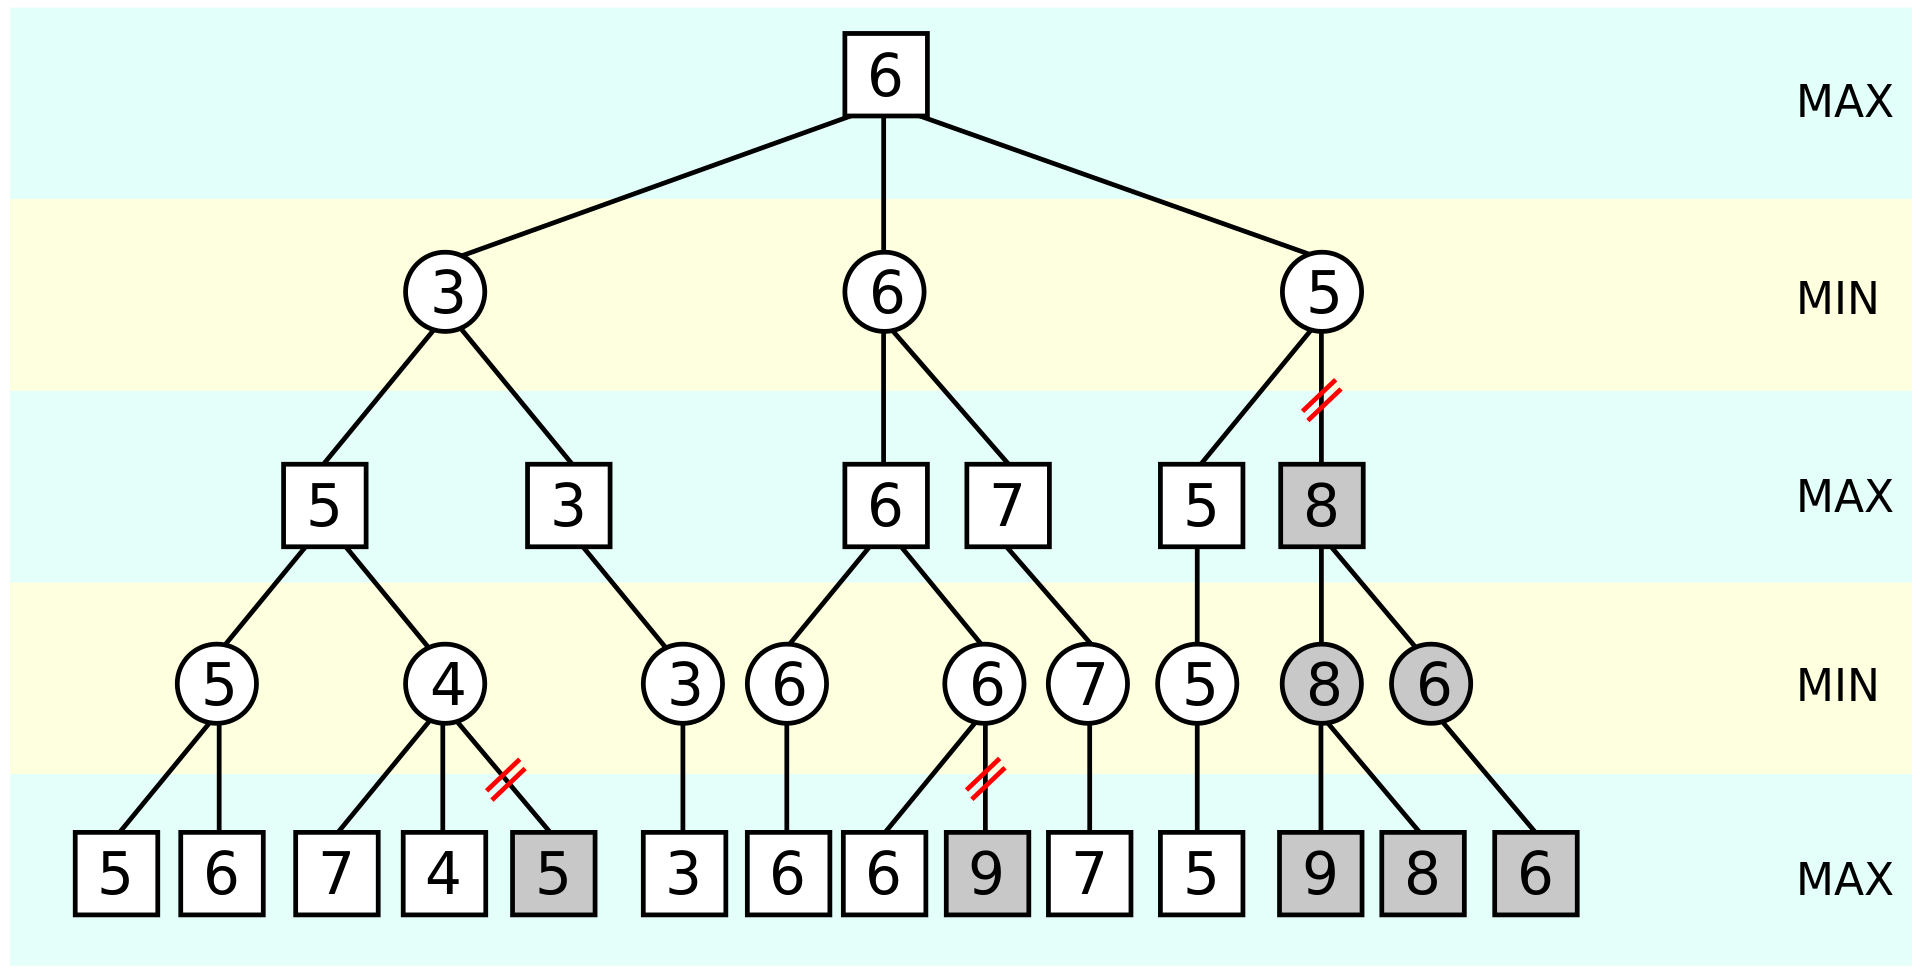
\includegraphics[width=0.7\textwidth]{ab.png}
		\caption{Exemple d'éxécution de l'algorithme alpha beta. Source: \url{https://commons.wikimedia.org/wiki/File:AB\_pruning.svg}}
\end{figure}

Dans cet exemple nous avons trois élagages qui ont eu lieu (tous les noeuds sont affichés évalués pour la clarté), de gauche à droite:\\
Nous cherchons à maximiser la valeur du noeud 5 à la profondeur 3 mais à minimiser la valeur de ses enfants.
Ainsi pour que le noeud 4 soit utile il faudrait que sa valeur puisse encore dépasser 5 (notre valeur d'$\alpha$) en explorant ses enfants. Or comme nous minimisons
sa valeur nous ne pourrons jamais dépasser 4, et par conséquent, ainsi il est inutile de continuer et d'valuer le noeud qui aurait valu 5.
Nous avons économisé une évaluation ici.\\
Nous cherchons ensuite à maximiser la valeur du noeud 6 à la profondeur 3 en minimisant la valeur de ses enfants.
Ainsi le second noeud 6 n'est intéressant que si il peut dépasser le 6 (notre valeur d'$\alpha$) déjà calculé, or c'est impossible pour la même raison
que précédemment, donc nous gagnons encore une évaluation.\\
Enfin, nous cherchons à minimiser le noeud 5 à la profondeur 2 tout en maximisant ses enfants.
Nous avons déterminé que sa valeur ne pouvais pas être supérieure à 5, or pour être utile il faudrait qu'elle puisse dépasser 6 (notre $\alpha$) pour 
remplacer la valeur du noeud 6 de profondeur 1. Ainsi il est inutile de regarder le reste de sons sous arbre car cette partie est inutile.
Nous gagnerons ici 6 évaluations.\\
Dans ce cas nous aurions évalué 33 noeuds avec le négamax et seulement 25 avec l'alpha beta, ce qui représente un gain non négligeable. Nous sommes loin 
de la valeur optimale théorique mais l'amélioration est conséquente et le sera de plus en plus lorsque la taille de l'arbre augmentera. \\

\pagebreak
Dans la même idée que précédemment pour passer du \textsc{Minimax} au \textsc{Négamax} nous pu adapter la procédure pour qu'elle soit correcte dans
notre framework négamax. L'algorithme est plus court mais pas forcément plus simple que la version reposant sur le minimax. Il est le suivant:\\
\begin{algorithm}
\caption{Algorithme de l'élagage alpha-beta}\label{negamax}
\begin{algorithmic}[1]
\Procedure{AlphaBeta}{$node, alpha, beta, depth$}
	\If{depth = 0}
		\State \textbf{return} \textsc{evaluate}$(node.move)$
	\EndIf
	\ForAll{child \textbf{in} node.children}
		\State score $\gets -\textsc{AlphaBeta}(child,-beta, -alpha, depth -1)$
		\If{score $>=$ beta}
			\State \textbf{return} beta
		\EndIf
		\If{score $>$ alpha}
			\State alpha $\gets$ score
		\EndIf
	\EndFor
	\State \textbf{return} alpha
\EndProcedure
\end{algorithmic}
\end{algorithm}

Comme pour le \textsc{Negamax} nous appelons initialement cette procédure depuis une version modifée qui récupérera la coup après la ligne 11.\\
Les paramètres $\alpha$ et $\beta$ seront respectivement initialisés à $-\infty$ et $+\infty$.\\
Une façon de réduire le nombre de noeuds évalués serait de considérer à la gauche de l'arbre (les coups évalués en premiers) les coups potentiellement
bons en choisissant une heuristique telle que la distance au centre du pion posé par le coup, car un coup a plus ce chance d'être bon si il est au centre.

\pagebreak
%==============================================================================
\section{Évaluation d'une position}

Tout d'abord, afin de respecter les conditions d'utilisation du framework Negamax, nous devons uen fonction d'évaluation asymétrique, elle sera définie
dans notre cas par: évaluation = évaluation(joueur courant) - évaluation(adversaire), ce qui respecte cette condition.\\
Notre évaluation sera basée de du pattern matching, avec un très grand nombre de patterns, mais tout d'abord nous devons vérifier si la partie est terminée
pour donner des scores signifiant la victoire (ou la défaite).

\begin{figure}[!hbt]
	\centering
	\begin{TAB}(e,0.5cm,0.5cm){|c|c|c|c|c|c|c|c|}{|c|c|c|c|c|c|c|c|}
		X &  &  &  &  &  &  &  \\
		 & X &  &  &  &  &  &  \\
		 &  &X  &  &  &  &  &  \\
		 &  &  &X  &  &  &  &  \\
		 &  &  &  &X  &  &  &  \\
		 &  &  &  &  &  &  &  \\
		 &  &  &  &  &  &  &  \\
		 &  &  &  &  &  &  &  
	\end{TAB}\hspace{0.5cm}
	\begin{TAB}(e,0.5cm,0.5cm){|c|c|c|c|c|c|c|c|}{|c|c|c|c|c|c|c|c|}
		X &  &  &  &  &  &  &  \\
		X &  &  &  &  &  &  &  \\
		X &  &  &  &  &  &  &  \\
		X &  &  &  &  &  &  &  \\
		X &  &  &  &  &  &  &  \\
		 &  &  &  &  &  &  &  \\
		 &  &  &  &  &  &  &  \\
		 &  &  &  &  &  &  &  
	\end{TAB}
	
	\begin{TAB}(e,0.5cm,0.5cm){|c|c|c|c|c|c|c|c|}{|c|c|c|c|c|c|c|c|}
		X & X & X & X & X &  &  &  \\
		 &  &  &  &  &  &  &  \\
		 &  &  &  &  &  &  &  \\
		 &  &  &  &  &  &  &  \\
		 &  &  &  &  &  &  &  \\
		 &  &  &  &  &  &  &  \\
		 &  &  &  &  &  &  &  \\
		 &  &  &  &  &  &  &  
	\end{TAB}\hspace{0.5cm}
	\begin{TAB}(e,0.5cm,0.5cm){|c|c|c|c|c|c|c|c|}{|c|c|c|c|c|c|c|c|}
		 &  &  &  & X &  &  &  \\
		 &  &  & X &  &  &  &  \\
		 &  & X &  &  &  &  &  \\
		 & X &  &  &  &  &  &  \\
		X &  &  &  &  &  &  &  \\
		 &  &  &  &  &  &  &  \\
		 &  &  &  &  &  &  &  \\
		 &  &  &  &  &  &  &  
	\end{TAB}
	\caption{Patterns vérifiés pour la victoire ou non}
\end{figure}

Afin de tester la victoire ou non, nous devons avoir 5 pions alignés, ce qui correspond à savoir si l'un des motifs ci dessus est présent dans le
plateau du joueur courant. Dans le cas où l'un serait présent nosu retournerons un score de 100000 qui correspondra à une valeur innateginable, mais
pas tout à fait l'infini, nous devons rester plus petit que les valeurs d'infini utilisées pour $\alpha$ et $\beta$ lors de l'élagage alpha beta.\\

Sinon, nous utiliserons des patternes similaires, notamment des lignes brisées, des lignes comme pour la victoire mais de longueur inférieure. Mais nous regarderons
aussi lorsque l'ennemi bloque notre avancée, comme par exemple pour une ligne drotie de 3 de longueur bloquée des deux côtés par notre adversaire.\\
Cependant il faut réussir à déterminer quels motifs sont importants à regarder car plus nous évaluons de motifs sur chaque position, moins nous pourrons
évaluer de positions en un temps imparti. Il faut donc faut trovuer le juste milieu entre quantité et qualité des motifs recherchés.\\

De plus certaines zones du plateau sont plus intéressantes d'un point de vue stratégique, notamment le centre, ainsi nous préférons jouer un pion au centre
du plateau plutôt que dans un coin. Nous matérialisons cette priorité de placement par la grille coefficientée suivante:
\pagebreak

\begin{figure}[!hbt]
		\center
	\begin{TAB}(e,0.5cm,0.5cm){|c|c|c|c|c|c|c|c|}{|c|c|c|c|c|c|c|c|}
		1 & 2 & 3 & 4 & 4 & 3 & 2 & 1 \\
		2 & 3 & 4 & 5 & 5 & 4 & 3 & 2 \\
		3 & 4 & 5 & 6 & 6 & 5 & 4 & 3 \\
		4 & 5 & 6 & 7 & 7 & 6 & 5 & 4 \\
		4 & 5 & 6 & 7 & 7 & 6 & 5 & 4 \\
		3 & 4 & 5 & 6 & 6 & 5 & 4 & 3 \\
		2 & 3 & 4 & 5 & 5 & 4 & 3 & 2 \\
		1 & 2 & 3 & 4 & 4 & 3 & 2 & 1 
	\end{TAB}
	\caption{Coefficients relatifs à la position sur le plateau}
\end{figure}

La valeur d'une case est alors inversement proportionnelle à sa distance euclidienne au centre. Cela va nous permettre de favoriser certaines positions
tout en en éliminant certaines qui seraient illogiques, par exemple lorsque le plateau est vide, nous ne voulons pas jouer la première case visitée
mais une bonne case, et bien que ce choix soit purement arbitraire il produit des résultats cohérents avec la stratégie qu'un humain utiliserait.\\

En combinant les patternes et cette grille nous arrivons a de très bons résultats, que ce soit en début de partie ou en fin de partie car nous arrivons
à la fois à évaluer correctement une position sur un plateau presque vide et sur un plateau presque rempli.\\

Ainsi bien que cette évaluation soit fondamentale pour avoir un bon algorithme, c'est la partie la plus subjective, car nous ne connaissons pas forcément 
la stratégie optimale. Bien que le jeu ai été très étudié sur une grille de 15 $\times$ 15 nous sommes sur une grille plus petite et certaines observations
ou stratégies ne sont pas transposables parfaitement.\\
De plus si nous voullions la meilleur fonction d'évaluation possible (bien qu'aucune ne soit la meilleure de manière absolue) il nous faudrait
étudier le jeu plus en profondeur pour voir émerger des patternes et des tratégies intéressante, ou, à la manière des concepterus d'IA d'échecs, collaborrer
avec d'excellents joueurs afin de transférer leur savoir à la machine.\\

Nous atteignons bien ainsi une limite de la fonction d'évaluation, elle ne pourra jamais être fondamentalement meilleure que nous car nous l'avons
programmé, et ainsi elle va imiter notre style de jeu. Ainsi si nous avons programmé une fonction d'évaluation mauvaise, la machine aura beau calculer bien 
plus rapidement que nous, nous serons toujours capable de gagner. Cependant si elle est bien programmée (ce qui va être dur à évaluer), l'avantage de la puissance
de calcul de la machine la fera nous dominer.

\pagebreak
%==============================================================================
\section{Conlusion}
\subsection{Résultats}

Pour nous mesurer à la machine, nous avons avons utilisé une profondeur de recherche de 4 et l'élagage alpha beta.\\
Le premier constat que nous avons pu faire est qu'il est presque impossible de gagner contre la machine, elle arive bien à prévoir nos coups
et notre victoire et nous empeche donc de l'atteindre. Ainsi la grande majorité des parties se sont terminées en égalité ou en victoire
de la machine lorsque nous avons commis des erreurs.\\
Un exemple de partie que nous avons réalisé que nous avons trouvé intéressante est le suivant:

\begin{figure}[!hbt]
	\centering
	\begin{TAB}(e,0.5cm,0.5cm){|c|c|c|c|c|c|c|c|}{|c|c|c|c|c|c|c|c|}
		 &  &  &  &  &  &  &  \\
		 &  &  &  &  &  &  &  \\
		 &  &  &  &  &  &  &  \\
		 &  &  &  &  &  &  &  \\
		 &  &  &  &  &  &  &  \\
		 &  &  &  &  &  &  &  \\
		 &  &  &  &  &  &  &  \\
		 &  &  &  &  &  &  & O 
	\end{TAB}\hspace{0.5cm}
	\begin{TAB}(e,0.5cm,0.5cm){|c|c|c|c|c|c|c|c|}{|c|c|c|c|c|c|c|c|}
		 &  &  &  &  &  &  &  \\
		 &  &  &  &  &  &  &  \\
		 &  &  &  &  &  &  &  \\
		 &  &  &  &  &  &  &  \\
		 &  &  &  & X &  &  &  \\
		 &  &  &  &  &  &  &  \\
		 &  &  &  &  &  &  &  \\
		 &  &  &  &  &  &  & O 
	\end{TAB}
	
	\begin{TAB}(e,0.5cm,0.5cm){|c|c|c|c|c|c|c|c|}{|c|c|c|c|c|c|c|c|}
		 &  &  &  &  &  &  &  \\
		 &  &  &  &  &  &  &  \\
		 &  &  &  &  &  &  &  \\
		 &  &  &  &  &  &  &  \\
		 &  &  &  & X &  &  &  \\
		 &  &  &  &  &  &  &  \\
		 &  &  &  &  &  &  &  \\
		 &  &  &  &  &  & O & O 
	\end{TAB}\hspace{0.5cm}
	\begin{TAB}(e,0.5cm,0.5cm){|c|c|c|c|c|c|c|c|}{|c|c|c|c|c|c|c|c|}
		 &  &  &  &  &  &  &  \\
		 &  &  &  &  &  &  &  \\
		 &  &  &  &  &  &  &  \\
		 &  &  &  &  &  &  &  \\
		 &  &  &  & X &  &  &  \\
		 &  &  &  &  &  &  &  \\
		 &  &  &  &  &  &  &  \\
		 &  &  &  & X &  & O & O 
	\end{TAB}
	\caption{Exemple de début de partie}
\end{figure}

Dans cette partie nous avons joué les O et la machine les X, comme nous pouvons le voir nous avosn vite été stoppés mais pas
de la manière la plus évidente.
Au lieu de venir se positionner directement devant nous, l'ordinateur a joué une case plus loin, ce uqi aura le même résultat 
pour nous limiter mais qui à moyen terme avantagera l'ordinateur car ses deux pions pourrons ainsi être reliés par une ligne droite.\\
Cette exemple illustre bien l'utilité de calculer en profondeur les coups car cela nous donne des stratégies comme celle ci qui se révèlent
très efficaces.\\

Cependant nous avons pu dans certains cas piéger la machine qui de temps en temps jouait de manière étonnante, en jouant toujours la case
correspondant au bit de poids faible du bitboard. Ceci est du à un bug dans notre code mais nous n'avons pas pu le trouver pour le résoudre à temps.\\
Mais lorsque cela se produit, l'ordinateur pense toujours à nous bloquer pour ne pas que nous gagnions la partie, donc même si ses chances de gagner
deviennent quasi-nulles, sa défaite n'est pas garantie.\\

\pagebreak
\subsection{Pour aller plus loin}

Comme nous avons pu le voir nous avons obtenu un résultat très satisfaisant, mais qui pourrait otujours être amélioré.\\
Tout d'abord la fonction d'évaluation pourrait l'être, que ce soit en réalisant plus de tests pour ajuster les différents motifs/poids,
ou en étudiant encore plus en détail les stratégies possibles pour gagner.\\

Mais la plupart des améliorations que nous pourrions réaliser sont plus liées à l'implémentation des algorithmes qu'aux algorithmes en eux mêmes.\\
Comme explicité plus haut, nous pourrions évaluer les positions dans un certain ordre pour réduire le nombre de noeuds évalués par l'élagage alpha
beta.\\
Nous pourrions aussi paralléliser l'évaluation des coups et le pattern matching afin de bénéficier des multiples coeurs présents sur nos machines.
Cela nous donnerait un gain de performance considérable et nous permettrait d'évaluer plus de positions, afin d'être encore meilleur qu'actuellement.\\

De manière ecore plus liée à l'implémentation, nous pourrions optimiser notre usage de la mémoire, limiter le nombre d'opérations, et profiter encore plus
de certaines opérations qui sont implémentée très efficacement, par exemples les opérateurs $>>$ et $<<$ sont implémentés au niveau hardware, ce qui les
rends très rapides.\\

Ainsi la majeure partie des améliorations des performances seraient du côté de la fonction d'évaluation pour augmenter la qualité de notre algorithme
et du côté de l'implémentation des nos algorithmes pour gagner en vitesse.
\pagebreak

\end{document}
